\section{Trabajo Relacionado} \label{sec:related_work_fair}

Los juegos estocásticos con funciones de \textit{payoff} han sido ampliamente investigados en la literatura. En \cite{FilarV96}, se presentan varios resultados sobre \emph{juegos transitorios},
una versión generalizada de juegos estocásticos terminantes con \textit{payoff} de recompensa total.
En los juegos transitorios, ambos jugadores poseen estrategias óptimas (sin memoria y deterministas).
Lo que es más importante, los juegos están determinados y su valor puede calcularse como el mínimo punto fijo de un conjunto de ecuaciones.
La mayoría de estos resultados se basan en el hecho de que el funcional $\Gamma$ (ver Sección \ref{sec:stopping_fair}) para juegos transitorios tiene un único punto fijo.
Tengamos en cuenta que en este capítulo hemos tratado con juegos que se detienen solo bajo supuestos de \textit{fairness}. Por lo tanto, el funcional correspondiente
puede tener varios puntos fijos. Por lo tanto, los principales resultados presentados en \cite{FilarV96} no se aplican a nuestro contexto.

\cite{DBLP:journals/fmsd/ChenFKPS13} y \cite{SvorenovaKwiatkowska16} presentan marcos lógicos para la verificación y síntesis de sistemas. Mientras que~\cite{DBLP:journals/fmsd/ChenFKPS13} proporciona una solución para una lógica temporal ramificada probabilística extendida con funciones objetivo de recompensa total, de descuento y de promedio esperado, \cite{SvorenovaKwiatkowska16} hace lo mismo en una extensión similar de una lógica probabilística temporal lineal. Ambos marcos se implementaron en la herramienta \Prism~\cite{DBLP:conf/cav/KwiatkowskaN0S20,DBLP:conf/cav/KwiatkowskaNP11}. Aunque en estos marcos se puede expresar una amplia clase de propiedades, ninguna de ellas se presenta bajo ambientes \textit{fair}. De hecho, estos trabajos son sobre juegos multijugador estocásticos en los que cada jugador es tratado por igual.

%% \cite{DBLP:journals/fmsd/ChenFKPS13} and \cite{SvorenovaKwiatkowska16} present logical frameworks for the verification and synthesis of systems.  While~\cite{DBLP:journals/fmsd/ChenFKPS13} presents a framework that combines a probabilistic branching temporal logic with expected total, discounted, and average reward objective functions, \cite{SvorenovaKwiatkowska16} does the same in the context of a probabilistic linear temporal logic. Both frameworks were implemented in the tool \Prism~\cite{DBLP:conf/cav/KwiatkowskaNP11}. Although a vast class of properties can be expressed in these frameworks, none of them are presented under fair environments.  In fact, these works are on stochastic multiplayer games in which each player is treated equally.

Sin embargo, de todos los operadores en ~\cite{DBLP:journals/fmsd/ChenFKPS13,SvorenovaKwiatkowska16,DBLP:conf/cav/KwiatkowskaN0S20}, $\langle \langle p_1 \rangle \rangle \ \textsf{R}_{\text{max}{=}?}[\textsf{F}^{\infty} T]$ es el mas cercano a nuestra propuesta y merece una comparación más profunda. $\langle \langle p_1 \rangle \rangle \ \textsf{R}_{\text{max}{=}?}[\textsf{F}^{\infty} T]$ devuelve la recompensa acumulada esperada hasta llegar a $ T$ en el que jugadas infinitas reciben un valor infinito~\cite{DBLP:journals/fmsd/ChenFKPS13,DBLP:conf/cav/KwiatkowskaN0S20}.
{\Prism} aproxima este valor calculando un punto fijo mayor. Utiliza un algoritmo de dos fases para hacerlo:
\begin{enumerate}[(i)]
\item%
  primero reemplaza las recompensas de valor cero con un pequeño valor positivo y aplica \textit{value iteration} en esta modificación para obtener un límite superior estimado, y
\item%
  este limite superior es usado para comenzar otro proceso de \textit{value iteration} destinado a computar el máximo punto fijo.
\end{enumerate}
%
\begin{figure}
%\vspace{-4ex}
%\fontsize{6.6}{6.6}\selectfont\ttfamily
\centering
\scalebox{0.9}{
  \begin{tikzpicture}[on grid,auto,align at top]
    \node[minvert] (v0)                   {$v_0(0)$};
    \node[probvert] (v6) [right=2.3 of v0] {$v_6(2)$};
    \node[probvert] (v8) [right=2.3 of v6] {$v_8(0)$};
    \node[probvert] (v7) [right=2.3 of v8] {$v_7(1)$};
    \node[probvert] (v1) [below=2.3 of v6] {$v_1(0)$};
    \node[probvert] (v2) [right=2.3 of v1] {$v_2(0)$};
    \node[probvert] (v3) [right=2.3 of v2] {$v_3(0)$};
    \node[probvert] (v4) [right=2.3 of v3] {$v_4(0)$};
    \node[maxvert] (v5) [right=2.3 of v4] {$v_5(0)$};
    
    \draw[rounded corners,->] (v0) -- (v1);
    \draw[rounded corners,->] (v0) -- (v6);
    \draw[rounded corners,->] (v6) -- (v8);
    \draw[rounded corners,->] (v7) -- (v8);
    \draw[rounded corners,->] (v1) -- (v2) node[midway] {$p$};
    \draw[rounded corners,->] (v2) -- (v3) node[midway] {$p$};
    \draw[rounded corners,->] (v3) -- (v4) node[midway] {$p$};
    \draw[rounded corners,->] (v4) -- (v5) node[midway] {$p$};
    \draw[rounded corners,->] (v5.north) -- ++(0,1) |- (v7.east);   
    \draw[rounded corners,->] (v5.south) -- ++(0,-1) -| (v1.south); 
    \draw[rounded corners,->] (v4.east) -- ++(0,-1.4) node[pos=0.5] {$1-p$} -| (v1.south) ;
    \draw[rounded corners,->] (v3.east) -- ++(0,-1.2) node[pos=0.5] {$1-p$} -| (v1.south);
    \draw[rounded corners,->] (v2.east) -- ++(0,-1) node[pos=0.5] {$1-p$} -| (v1.south);
    \draw[rounded corners,->] (v1.east) -- ++(0,-0.8) node[pos=0.5] {$1-p$} -| (v1.south);
  \end{tikzpicture}
  }
%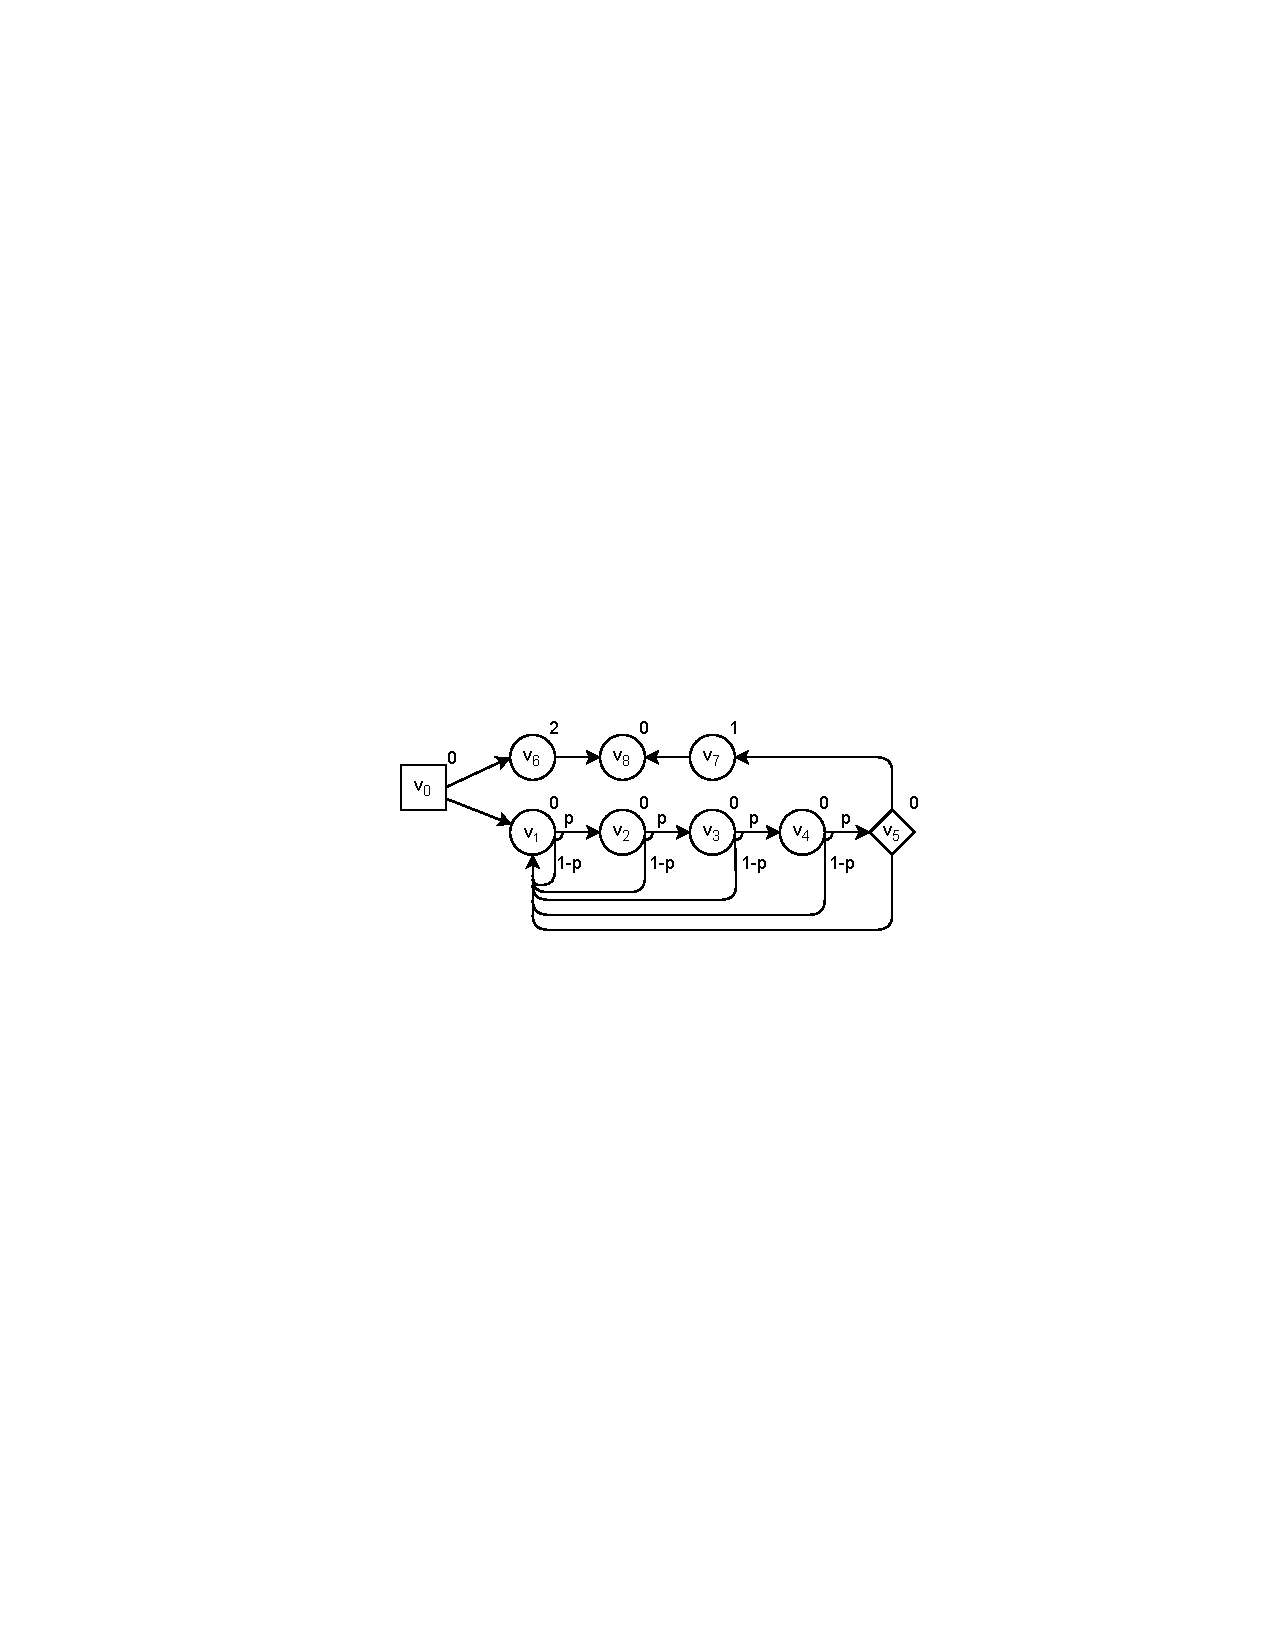
\includegraphics[scale=0.80]{Figs/prism-cex-1-horiz.pdf}%\hspace{1.5em}\mbox{}
\caption{Un simple juego de 2 jugadores: solo se muestran las probabilidades menores a 1.} \label{fig:prism-cex-1}
\end{figure}
Esta heurística podría devolver aproximaciones erróneas del mayor punto fijo. Ilustramos esto con un ejemplo sencillo. Considere el juego representado en la Figura~\ref{fig:prism-cex-1}. Para cualquier $\textsf{p}$, el valor del punto fijo más grande en el vértice $v_0$ es $2$. Sin embargo, al tomar $\textsf{p}=0.99$ y la tolerancia $\epsilon=10^{-6}$, {\Prism} devuelve un valor cercano a $39608$. %el valor $39607.955145476146$.
Esto ocurre porque {\Prism} cambia $0$ al valor $0.02$, lo que da como resultado un límite superior extremadamente grande.
%% Además, cada iteración solo produce una pequeña modificación en los valores %lo que arroja un valor final erróneo
%% lo que conduce a una convergencia incorrecta.
Obviamente, también devuelve una estrategia incorrecta para el vértice $v_0$. Hemos comprobado este ejemplo con nuestra herramienta y devolvió el valor correcto para el vértice $v_0$ en $2$ iteraciones, independientemente del valor de $\textsf{p}$.
%
Hemos elegido un valor grande para $\textsf{p}$ para que la diferencia sea notable. Los valores pequeños también pueden producir valores diferentes en, por ejemplo, $\textsf{v}_1$ solo que podría atribuirse a errores de aproximación.
%
%% Varying the relative error does not yield a better solution. In fact, taking $\epsilon = 10^{-8}$ {\Prism} returns a value closer to $2010051$.
%% \remarkPRD{Saque lo de las iteraciones porque no creo que agregue nada}
%% %a value of $2010050.7754585734$,  and also the number of iterations needed to compute such a value is increased: {\Prism} took $69508550$ iterations and $~30$ seconds with $\epsilon=10^{-8}$.}
%% Similar examples can be built to show that the upper bound estimated by {\Prism} could return a value smaller than the greatest fixpoint, yielding an incorrect final value.
%
También ejecutamos este operador en nuestros casos de estudio y observamos pequeñas diferencias en muchos de ellos (particularmente en Roborta) que aumentan cuando las probabilidades de falla también aumentan.




%% \subsection{{\Prism} Operators.} {\Prism} supports 2-player stochastic games,  therein properties are specified via the logic $\text{rPATL}$.This logic provides operators for expected rewards. Most of these operators are computed via a least fixpoint; thus, they are not comparable with our approach (they return $0$ in the case of a $0$-valued cycles).
%% Interestingly,  the operator  $\langle \langle p_1 \rangle \rangle \ \textsf{R}_{\text{max}{=}?}[\textsf{F}v]$ \remarkPRD{cambi\'e esto. Antes dec\'ia $\langle \langle p_1 \rangle \rangle \text{min}{=}?\textsf{R}[\textsf{F}v]$. Fijense que cambi\'e ``min'' por ``max''} returns the expected accumulated reward in which infinite plays receive an infinite value~\cite{DBLP:journals/fmsd/ChenFKPS13,DBLP:conf/cav/KwiatkowskaN0S20}.  {\Prism} approximates this value by computing a greatest fixpoint.  It uses a two-phase algorithm to do so:
%% \begin{enumerate}[(i)]
%% \item%
%%   it first replaces $0$-rewards by a small positive value and applies value iteration on this modification to get an estimated upper bound, and
%% \item%
%%   this upper bound is used to start another value iteration process aimed to compute the greatest fixpoint.
%% \end{enumerate}
%% %
%% \begin{wrapfigure}[10]{r}{55mm}
%% \vspace{-4ex}
%% %\fontsize{6.6}{6.6}\selectfont\ttfamily
%% \centering
%% 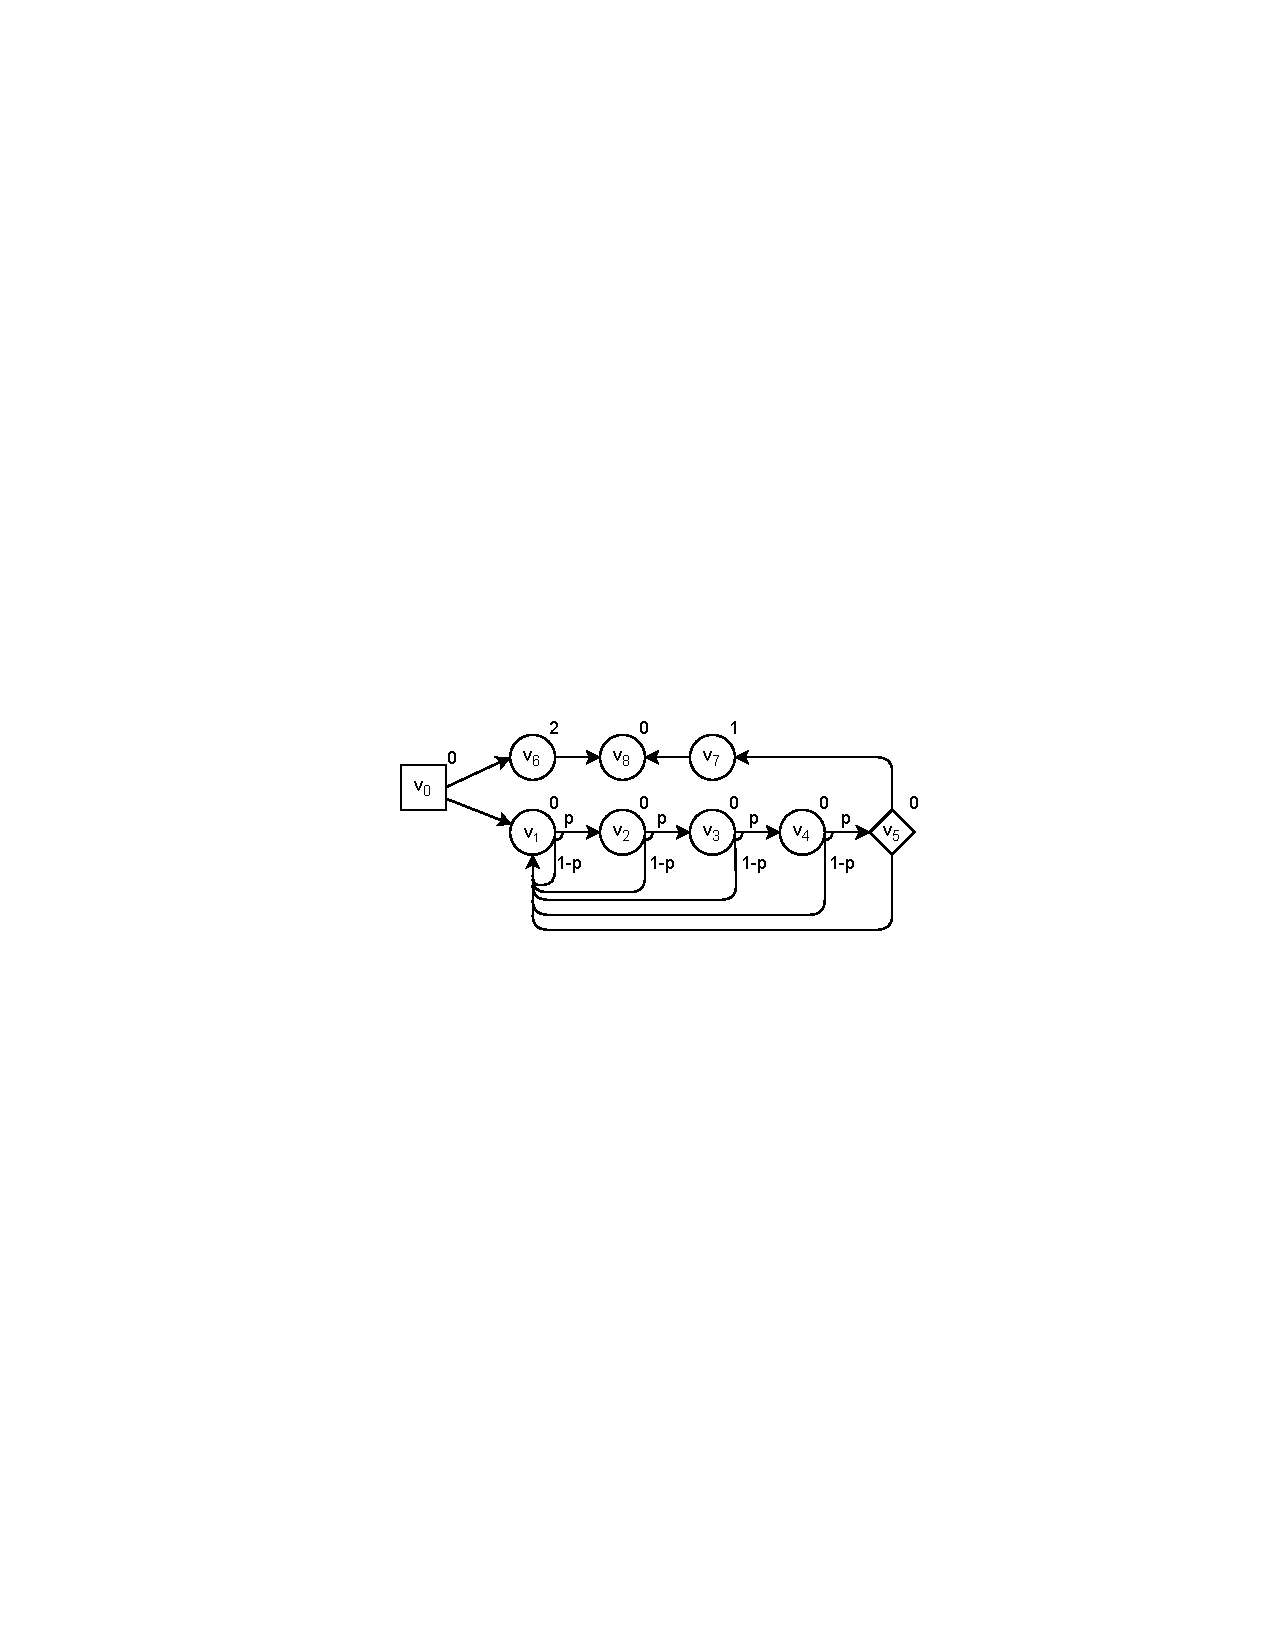
\includegraphics[scale=0.60]{Figs/prism-cex-1-horiz.pdf}%\hspace{1.5em}\mbox{}
%% \caption{A simple 2-player game: only probability less than 1 are shown.} \label{fig:prism-cex-1}
%% \end{wrapfigure}
%% This heuristic could return erroneous approximations of the greatest fixpoint.  We illustrate this with a simple example. Consider  the game depicted in Fig.~\ref{fig:prism-cex-1}, For any $T$, the value of the greatest fixpoint in vertex $v_0$ is $2$. However, by taking $T=0.99$ and tolerance $\epsilon=10^{-6}$, {\Prism} returns a value close to $39608$. %the value $39607.955145476146$.
%% This occurs because  {\Prism} changes $0$ by the value $0.02$, which results in an extremely large upper bound.  Furthermore, every iteration only produces a small modification in this value which yields an erroneous final value which leads to an incorrect convergence.   Obviously, it also returns an incorrect strategy for vertex $v_0$.  We have checked this example with our tool, and it returned the correct value for  vertex $v_0$ in $2$ iterations.
%% %
%% Varying the relative error does not yield a better solution. In fact, taking $\epsilon = 10^{-8}$ {\Prism} returns a value closer to $2010051$.
%% \remarkPRD{Saque lo de las iteraciones porque no creo que agregue nada}
%% %a value of $2010050.7754585734$,  and also the number of iterations needed to compute such a value is increased: {\Prism} took $69508550$ iterations and $~30$ seconds with $\epsilon=10^{-8}$.}
%% Similar examples can be built to show that the upper bound estimated by {\Prism} could return a value smaller than the greatest fixpoint, yielding an incorrect final value.


















Los \emph{Juegos estocásticos de camino mas corto} \cite{PatekBertsekas99} son juegos estocásticos de dos jugadores con recompensas (negativas o positivas) en los que las estrategias del minimizador se clasifican en \emph{adecuadas} e \emph{inadecuadas},
las estrategias adecuadas son las que aseguran la terminación. Como se demuestra en \cite{PatekBertsekas99}, estos juegos están determinados y ambos jugadores poseen estrategias óptimas sin memoria. Para probar estos resultados, los autores asumen que el valor esperado del juego para estrategias inadecuadas es $\infty$, esto asegura que el funcional correspondiente es una contracción y por lo tanto tiene un punto fijo único. Por el contrario, nos restringimos a recompensas no negativas pero no hacemos suposiciones sobre estrategias \textit{unfair}, como se mencionó anteriormente, la función correspondiente para nuestros juegos puede tener varios puntos fijos. Además, probamos que el valor del juego viene dado por el mayor punto fijo de $\Gamma$. En los últimos años, varios autores han investigado problemas estocásticos de camino más corto para MDPs (es decir, juegos de un solo jugador), donde se relaja la suposición sobre estrategias inadecuadas (por ejemplo, \cite{DBLP:conf/lics/Baier0DGS18}); hasta donde sabemos, estos resultados no se han extendido a los juegos de dos jugadores.

%% In \cite{SvorenovaKwiatkowska16}, a logical framework is presented for the verification and synthesis of systems. This framework combines probabilistic linear temporal logic with expected total, discounted, and average reward objective functions. 	The framework is implemented in the tool \Prism~\cite{DBLP:conf/cav/KwiatkowskaNP11}. Although a vast class of properties can be expressed in this framework, fairness assumptions over the environment are not dealt with in this line of research.
	
En \cite{DBLP:conf/ifipTCS/BolligC04} los autores abordan el problema de sintetizar un controlador que maximiza la probabilidad de satisfacer una propiedad {\LTL}. Las estrategias de \textit{fairness} se utilizan para reducir este problema a la síntesis de un controlador que maximiza una propiedad {\PCTL} sobre un juego producto. Sin embargo, este artículo no aborda las recompensas esperadas y la determinación del juego bajo supuestos de \textit{fairness}.

Curiosamente, en \cite{DBLP:conf/fossacs/AsarinCV10} los autores consideran el problema de ganar un juego de dos jugadores (no estocástico) con suposiciones de \textit{fairness} sobre el entorno. El objetivo del sistema es garantizar una propiedad $\omega$-regular. Los autores muestran que ganar en estos juegos es equivalente a ganar casi-seguramente en un proceso de decisión de Markov. Cabe señalar que este trabajo solo considera juegos no estocásticos. Además, las funciones de \textit{payoff} no se consideran allí.
%% Interestingly, in \cite{DBLP:conf/fossacs/AsarinCV10} the authors consider the problem of winning a (non-stochastic) two-player games with fairness assumptions over the environment. The objective of the system is to guarantee an $\omega$-regular property. The authors show that winning in these games is equivalent to almost-sure winning in a Markov decision process. It must be noted the aforementioned work only considers non-stochastic two-player games.  Furthermore, payoff functions are not considered therein.


        
%	The games introduced in \cite{Bacci0LM17,BacciBLMTB19,DesharnaisGJP04,DesharnaisLT11}  are based on probabilistic bisimulation, so they are symmetric. Furthermore, in \cite{DesharnaisGJP04,DesharnaisLT11} the nodes of the game graph are modeled using subsets of states of the PTSs, in our formulation
%we do not use subsets of states. The games defined in \cite{Bacci0LM17,BacciBLMTB19} use Kanterovich's and Hausdorff's liftings to deal with probabilistic distributions and non-determinism, respectively. In addition, the authors use the vertices of the transportation polytopes to model the probabilistic vertices. In contrast, we introduced a symbolic representation of games to avoid the state explosion caused by the vertices of the polytopes. Also note that the metrics introduced in \cite{Bacci0LM17,BacciBLMTB19} measure the (probabilistic) bisimulation distance between two PTSs, which for almost-sure failing systems is always $1$.
%		
%Another related framework is  defined in \cite{LanotteMT17}. Therein, the authors introduce a notion of weak simulation quasimetric tailored for reasoning about the evolution of \emph{gossip protocols}. This makes possible to compare network protocols that have similar behaviour up to a certain tolerance; being $0$ and $1$ the minimum and maximum distance, respectively.  Note that using this quasimetric to compare a network protocol with an almost-sure failing implementation will always return $1$, thus that approach cannot be used to quantify the masking fault-tolerance of almost-sure failing systems.
% 
% Finally, let us compare our approach with some metrics usual in fault-tolerance. \emph{Mean-Time To Failure} (MTTF) and \emph{Mean-Time Between Failures} (MTBF) \cite{ReliabilityBook}  capture the amount of time that a system is expected to be operative until it fails, and the expected elapsed time between failures, respectively.  These metrics are designed for hardware or electronic systems, where we have at hand estimations about the failure rate of the physical components. Our framework is designed to be used at a higher level of abstraction, where we have a model of the system to be implemented acting as a specification, and several possible implementations of it, described as probabilistic automata. This level of abstraction makes it possible to use this framework to analyze software fault-tolerance. Furthermore, note that our framework is particularly tailored to deal with masking fault-tolerance, a particular kind of fault-tolerance; in addition, our game formulation allows us to analyse systems on worst-case scenarios.

%\spnewtheorem*{proofofclaim}{Proof of claim}{\itshape}{\rmfamily}








%% \begin{proof}[of Theorem~\ref{thm:stopping-algorithm}]
%%   Recall the definitions of operators $\Apre$ and $\Epre$ for a given MDP $\MDP{H} = (V' , (V'_1,\emptyset, V'_\Probabilistic), \delta') $.
%% \begin{align*}
%% 	\Epre(C) \ = \ {}& \{ v \in V' \mid \delta'(v,C) > 0\} \\
%% 		      % & \cup \{ v \in  V'_1   \mid \exists v' \in V' : \delta'(v,v') * \delta(v', C) >0 \}\\
%% 	\Apre(C) \ = \ {} &\{ v \in V'_\Probabilistic  \mid \delta'(v,C) > 0\}
%% 		       \ \cup \ \{ v \in  V'_1   \mid \forall v' \in V' : \delta'(v,v') > 0 \Rightarrow v' \in C \}
%% \end{align*}
%% %
%% Furthermore, by considering that terminal vertices are absorbing, and let $T'$ be the terminal vertices of $\MDP{H}$, by Lemma 10.111 in~\cite{BaierK08}, we have that:
%% $\forall \strat{1} \in \Strategies{1}: \MDPProb{\strat{1}}_{\MDP{H},v}(\Diamond T') = 1$ iff $\inf_{\strat{1} \in \Strategies{1}} \MDPProb{\strat{1}}_{\MDP{H},v}(\Diamond T') = 1$ iff $v \in V' \setminus \Epre^*(V' \setminus \Apre^*(T'))$. 

%% %\remarkPC{add cite to Pedro's slides}\remarkPRD{Ah\'i puse la referencia apropiada}

%% Now, consider the MDP $\StochG^{\uniformstrat{2}}$, where $\uniformstrat{2}$ is the strategy defined in Theorem \ref{thm:uniform-prob}. Since $\uniformstrat{2}$ is memoryless, $\StochG^{\uniformstrat{2}}$ has the same vertices as $\StochG$ (the vertices in $V_2$ are considered as probabilistic vertices). Furthermore, note that $v \in  \AFairpre^*(C)$ (in game $\StochG$) iff
%% $v \in  \Apre^*(C)$ (in MDP $\StochG^{\uniformstrat{2}}$).
%% Then, $ v \in V\setminus \AFairpre^*(C)$ (in game $\StochG$) iff $v \in V \setminus \Apre^*(C)$ (in MDP $\StochG^{\uniformstrat{2}}$). 
%% That is, $ v \in \EFairpre^*(V \setminus \AFairpre^*(C))$ (in game $\StochG$)
%% iff $ v \in \Epre^*(V \setminus \Apre^*(C))$ (in MDP $\StochG^{\uniformstrat{2}}$), since $\Epre^*(S)$ and $\EFairpre^*(S)$ also coincide over 
%% any set of vertices. By the aforementioned property of MDPs, we have: 
%%  $\Prob{\strat{1}}{\uniformstrat{2}}_{\StochG,v}(\Diamond T) = 1$ for every $\strat{1} \in \Strategies{1}$  iff
%% $v \in \EFairpre^*(V \setminus \AFairpre^*(T))$. The  result follows by Theorem \ref{sec:fair-strats}.
%% \end{proof}